\chapter{Deep Learning and Convolutional Representations}

Depth became central in machine learning once practitioners learned how to train large models and once data and compute became abundant enough for those models to be useful. The point of depth is not mystery. It is representation: deeper models can construct progressively more abstract features.

\section{Why depth helps}

In a deep feedforward network, repeated composition produces
\[
  \hvec^{(L)}
  =
  f_L \circ f_{L-1} \circ \cdots \circ f_1(\vec{x}).
\]
Each layer reshapes the representation seen by the next layer. This can be far more parameter-efficient than forcing one shallow layer to realize the same input--output map directly \parencite{goodfellow2016deep,hastie2009elements}.

\begin{aside}[Trainability is separate from expressivity]
Universal approximation tells us that shallow networks can represent many functions. It does not say that those functions are easy to learn from finite data with finite computation.
\end{aside}

\section{Vanishing gradients and practical remedies}

Deep networks were historically difficult to train because repeated chain-rule multiplication can shrink or amplify gradients exponentially. If each local derivative has magnitude below one, gradients decay with depth; if it exceeds one, they can explode.

Several practical changes broke this bottleneck:
\begin{itemize}
  \item non-saturating nonlinearities such as ReLU,
  \item better initialization,
  \item normalization and adaptive optimization,
  \item pre-training in earlier deep-learning practice,
  \item larger datasets and hardware acceleration.
\end{itemize}

\section{Hierarchical features}

\begin{figure}[t]
\centering
\IfFileExists{figures/deep-representation-ladder.png}{%
  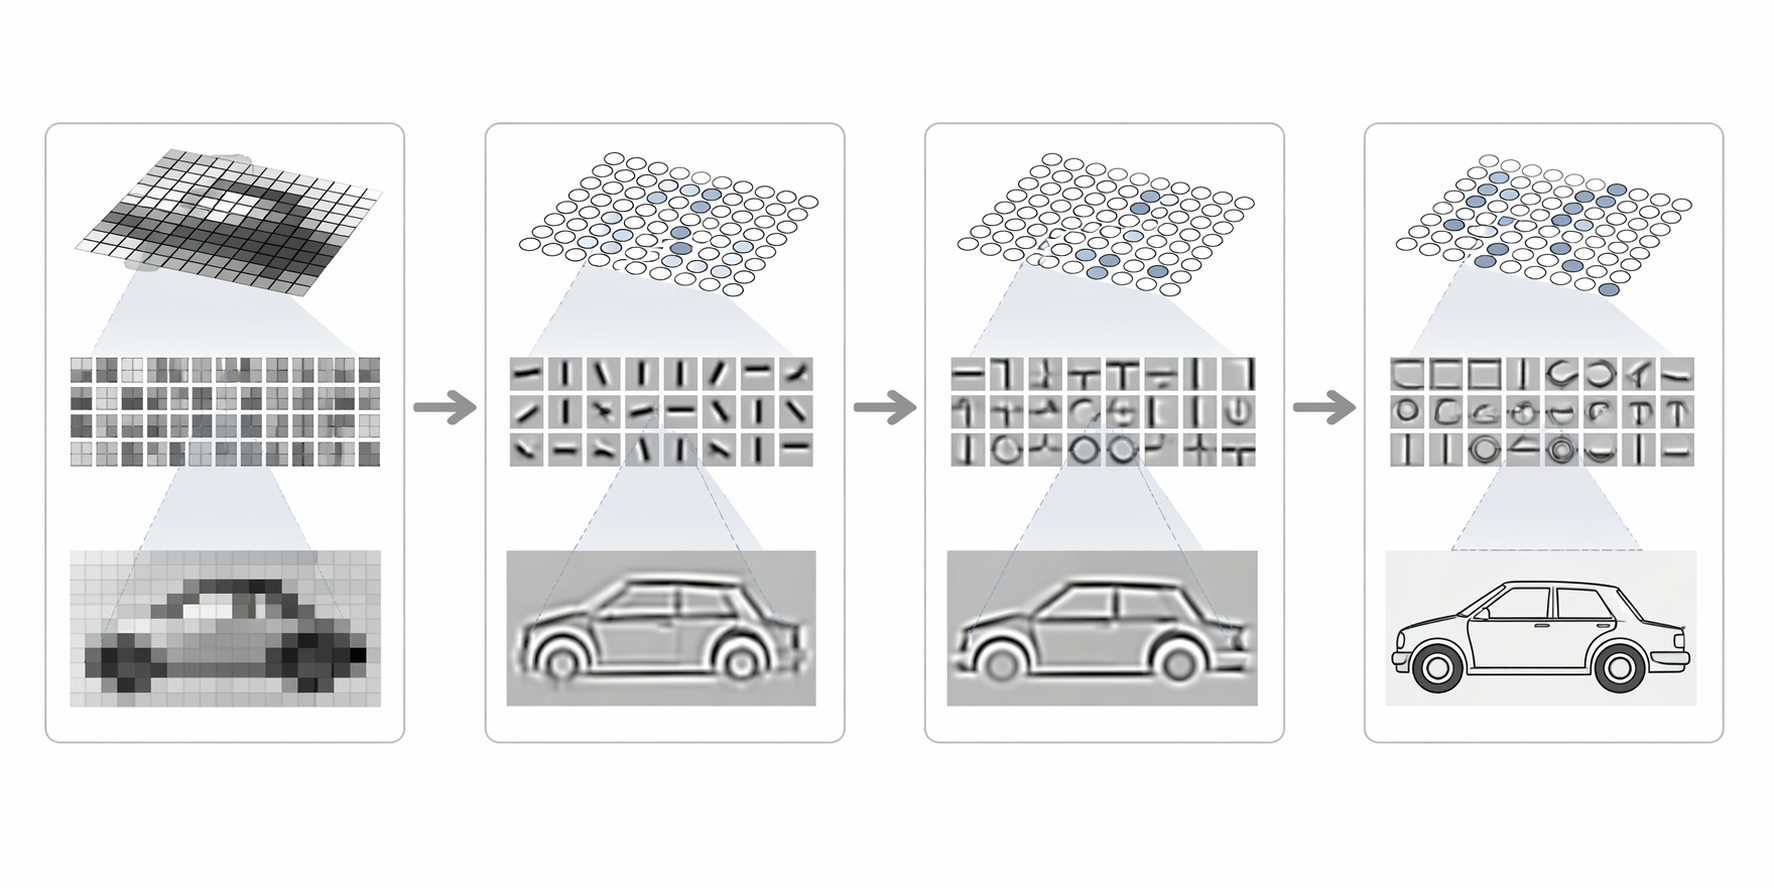
\includegraphics[width=0.88\textwidth]{figures/deep-representation-ladder.png}
}{%
  \begin{tikzpicture}[node distance=2.2cm]
    \node[draw, minimum width=2.4cm, minimum height=1.5cm] (p1) {pixels};
    \node[draw, minimum width=2.4cm, minimum height=1.5cm, right=of p1] (p2) {edges};
    \node[draw, minimum width=2.4cm, minimum height=1.5cm, right=of p2] (p3) {parts};
    \node[draw, minimum width=2.4cm, minimum height=1.5cm, right=of p3] (p4) {objects};
    \draw[->, very thick] (p1) -- (p2);
    \draw[->, very thick] (p2) -- (p3);
    \draw[->, very thick] (p3) -- (p4);
  \end{tikzpicture}
}
\caption{Representative deep-learning intuition: successive layers transform raw input into progressively more abstract features. When the Codex-generated figure is present, it replaces the schematic fallback.}
\end{figure}

The intuitive picture is a hierarchy:
\begin{itemize}
  \item early layers capture local regularities,
  \item intermediate layers combine them into motifs or parts,
  \item late layers encode task-relevant abstractions.
\end{itemize}
This is why depth often helps even when the final task is ``just'' classification: the network is learning a useful internal language for the data.

\section{Autoencoders and pre-training}

An autoencoder learns an encoder $g_\phi$ and decoder $h_\psi$ so that
\[
  \vec{x} \approx h_\psi\!\bigl(g_\phi(\vec{x})\bigr).
\]
If the latent representation is lower-dimensional or otherwise constrained, the model must preserve the information that matters most for reconstruction. Earlier deep-learning practice used such objectives for unsupervised pre-training; the broader lesson survives even today: representation learning can be useful before the final supervised task is optimized.

\section{Convolutional layers}

Images and other grid-structured signals have strong locality and approximate translation symmetry. Convolutional layers exploit that structure by sharing one local filter across positions. In two dimensions,
\[
  (\mat{K} * \mat{X})_{ij}
  =
  \sum_{u,v} K_{uv} X_{i-u,j-v}.
\]

\begin{keyequation}[Why convolution works]
\[
  (\mat{K} * \mat{X})_{ij}
  =
  \sum_{u,v} K_{uv} X_{i-u,j-v}
\]
\tcblower
The same filter is reused at every position. This drastically reduces parameter count and biases the network toward local feature detection.
\end{keyequation}

Pooling layers then summarize nearby activations, which improves robustness to small shifts and deformations. The key inductive bias is not that CNNs are universally better, but that they are matched to data with local correlation structure.

\section{Regularization in deep networks}

Deep models remain vulnerable to overfitting, so the usual tools reappear in more specialized form:
\begin{itemize}
  \item \textbf{data augmentation}: enlarge the effective dataset by label-preserving transformations,
  \item \textbf{dropout}: prevent units from depending too strongly on specific partners,
  \item \textbf{weight decay and early stopping}: still essential.
\end{itemize}

The deep-learning message of the course is therefore not ``depth solves everything.'' It is: depth is powerful when architecture, optimization, and data geometry are aligned.
